\documentclass{article}


% if you need to pass options to natbib, use, e.g.:
%     \PassOptionsToPackage{numbers, compress}{natbib}
% before loading neurips_2023


% ready for submission
% \usepackage{neurips_2023}
\usepackage[preprint]{neurips_2023}

% to compile a preprint version, e.g., for submission to arXiv, add add the
% [preprint] option:
%     \usepackage[preprint]{neurips_2023}


% to compile a camera-ready version, add the [final] option, e.g.:
%     \usepackage[final]{neurips_2023}


% to avoid loading the natbib package, add option nonatbib:
%    \usepackage[nonatbib]{neurips_2023}

\usepackage[utf8]{inputenc} % allow utf-8 input
\usepackage[T1]{fontenc}    % use 8-bit T1 fonts
\usepackage{hyperref}       % hyperlinks
\usepackage{url}            % simple URL typesetting
\usepackage{booktabs}       % professional-quality tables
\usepackage{amsfonts}       % blackboard math symbols
\usepackage{nicefrac}       % compact symbols for 1/2, etc.
\usepackage{microtype}      % microtypography
\usepackage{xcolor}         % colors
\usepackage{graphicx}

\title{Progress Report: \\ Subclaim Generation and Generative Retriever for Efficient Multi-Hop Fact Verification}


% The \author macro works with any number of authors. There are two commands
% used to separate the names and addresses of multiple authors: \And and \AND.
%
% Using \And between authors leaves it to LaTeX to determine where to break the
% lines. Using \AND forces a line break at that point. So, if LaTeX puts 3 of 4
% authors names on the first line, and the last on the second line, try using
% \AND instead of \And before the third author name.


\author{%
  Saeyoung Choi \\
  \texttt{saeyoung.choi@snu.ac.kr} \\
  \And
  Jinwha Jang \\
  \texttt{gdejin@snu.ac.kr}
  \And
  Yan GuangJing \\
  \texttt{mysnuguangjing@snu.ac.kr} \\
}

\begin{document}

\maketitle

\section{Introduction}
As the cost of generating and delivering texts decreases, identifying misinformation and fact-checking becomes more important issues. Automatically generated misinformation is threatening to pollute the Internet. However, it is almost impossible to manually check the factuality of a massive number of texts generated by bots or language models. Hallucinations, plausible but incorrect text generation by language models, are also a difficult challenge to solve. Thus, the need for automated fact verification is urgent. With advances in natural language processing, attempts are being made to use various machine learning models for automatic fact verification \cite{chopra2017towards,zhong2019reasoning,nie2019combining}.\par
Recently, retrieval-augmented generation (RAG) \cite{lewis2020retrieval,izacard2020leveraging} is drawing attention for its potential in improving factuality of the language models \cite{shuster2021retrieval,ren2023investigating}. It can not only improve factuality but also provide explainability of the generated results, by utilizing both LLM's prior knowledge (parameters) and external knowledge (retrieved document). However, it is difficult to verify complex multi-hop claims. Also, constructing a reliable knowledge base and searching through it is expensive.\par
In this study, we propose a generative approach to enhance the model performance and efficiency, by utilizing generative capability of the language model for not only claim verification, but also querying and retrieval. This approach includes (1) subclaim generation to verify the complex factuality within multi-hop claims (like chain-of-thought approach) and (2) generative retrieval to dynamically obtain relevant evidence for each claim. We will integrate these two approaches into our baseline model, and evaluate the performance of the integrated model.


\section{Related Work}

\subsection{QACHECK : A Demonstration System for Question-Guided Multi-Hop Fact-Checking}
QACHECK \cite{pan2023qacheck} emerges as a groundbreaking model in the realm of automated fact verification, particularly within natural language processing (NLP). It innovatively adopts a question-guided multi-hop reasoning framework, significantly enhancing the clarity and effectiveness of fact-checking processes. Unlike traditional models that rely on linear evidence assessment, QACHECK dissects complex claims into simpler components through a series of contextually relevant questions. This methodology not only increases the interpretability of the verification process but also aligns closely with human cognitive patterns in assessing veracity. \par

\begin{figure}[h]
  \centering
  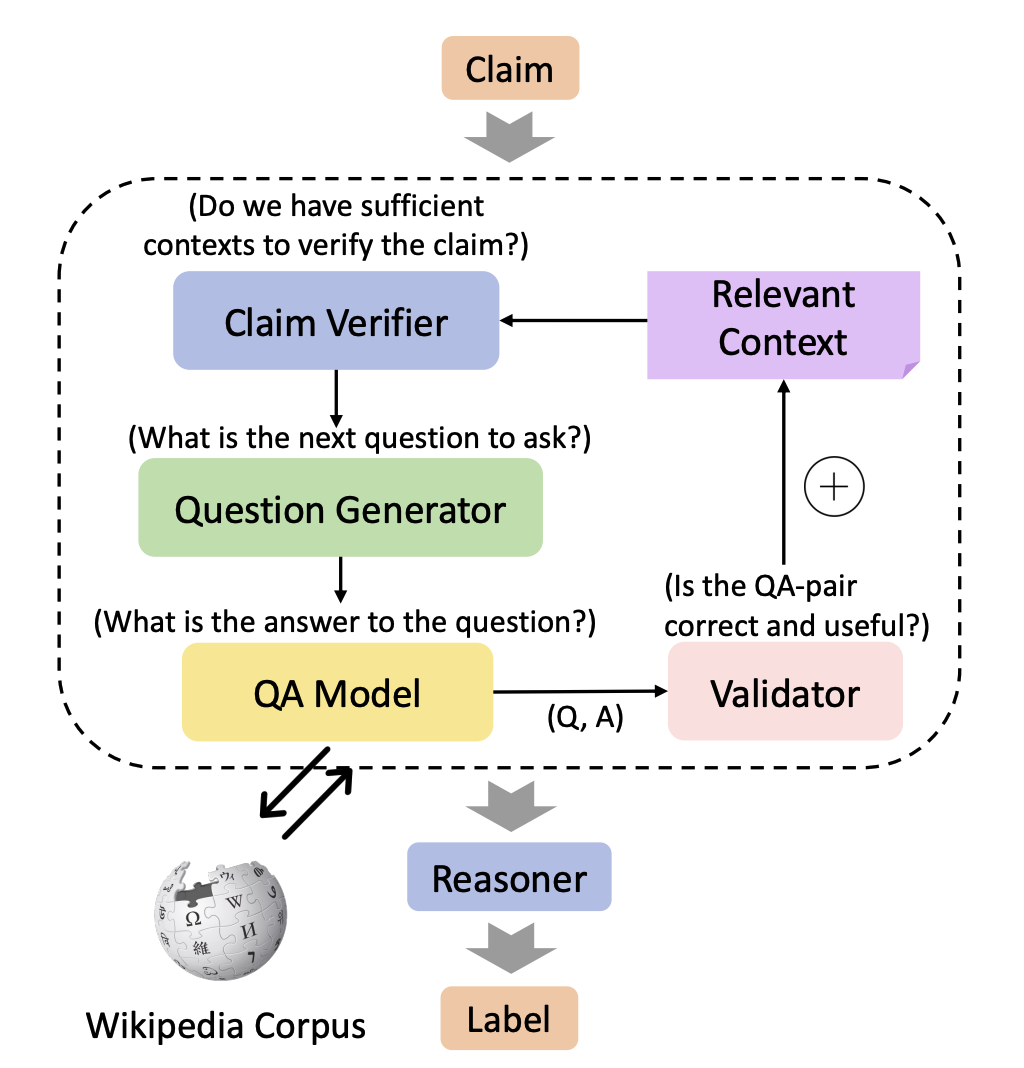
\includegraphics[width=0.4\linewidth]{Figure/Fig3.png}
  \caption{The Architecture of the QACHECK System}
\end{figure}

The architecture of QACHECK is a composite of five key modules: a claim verifier, a question generator, a question-answering module, a QA validator, and a reasoner. Each module plays a distinct yet interdependent role in the fact-checking pipeline. The claim verifier initially assesses the sufficiency of available context in substantiating a claim. Sequentially, the question generator and the QA module collaboratively work to explore and fill informational gaps. This synergy ensures a comprehensive examination of claims, thereby enhancing the accuracy of verification. \par
QACHECK's methodological innovation lies in its unique use of question-answer pairs for evidence validation, a significant deviation from conventional fact-checking models. By iteratively generating and validating these pairs, the model effectively accumulates a robust evidence base for each claim. This approach is particularly adept at tackling claims requiring deep, multi-faceted reasoning, a common challenge in NLP tasks focused on misinformation and fact verification. The integration of these components into a cohesive system offers a more transparent, user-friendly, and dynamic fact-checking process, addressing the ever-growing complexities in discerning factual accuracy in digital content.


\subsection{Generative Retrieval Models}
In previous works, most of the generative models applied to the information retrieval domain obey the “index-retrive-then-rank” principle. Such as the re-implementation of BERT for query-based passage re-ranking proposed by Nogueira et al. \cite{nogueira2019passage} as well as the DPR \cite{karpukhin2020dense} method used in the RAG model’s retriever. However, this kind of classical approach requires a large document index and a complicated search process, which leads to considerable memory and computational overhead. Additionally, independent scoring and ranking paradigms lack dependent information among documents and sentences. A fixed number of selected sentences are not precise in most cases and can result in lower accuracy.  \par
To mitigate these limitations, Chen et al. \cite{chen2022gere} proposed Generative Evidence Retrieval for Fact Verification (GERE) to adapt a pre-trained sequence-to-sequence model to dynamically select a precise set of relevant evidence for each claim by modeling the dependency among documents and sentences. 

\begin{figure}[h]
  \centering
  \includegraphics[width=0.5\linewidth]{Figure/Fig4.png}
  \caption{The Overview of the GERE Framework}
\end{figure}

GERE consists of 3 independent components, including claim encoder, title decoder and evidence decoder. It first encodes the claim into a compact vector with BART to capture its essential topics. Then the title decoder predicts a sequence of document titles based on both the claim and previous generated titles, here Beam Search is adopted for token prediction to save computational resources. Generated titles are used to retrieve relevant documents which contribute to a candidate sentence set. The sentence set are used to predict sentence identifiers, which generates a dynamic set of evidence. \par
The experimental results on FEVER dataset \cite{thorne2018fever} gives the best performance in terms of precision and F1 score, but fails in recall for sentence retrieval. This indicates that GERE provides a more compact but more preciser evidence set. Besides, GERE has a significant reduction of memory footprint and inference time of document retrieval, suggesting that it is much more resource-saving than other baseline models. By combining GERE with LLM, we hypothesize that our model can generate a more consistent output with less resource demand.

\section{Model Description}

\subsection{Model Overview}
\autoref{bl} and \autoref{pp} shows the architecture of our baseline model and proposed model, respectively. While the baseline model has conventional retriever and claim verifier, our proposed model consists of the following modules: (1) subclaim generator, (2) generative retriever (evidence generator), and (3) claim verifier. 

\begin{figure}[h]
  \centering
  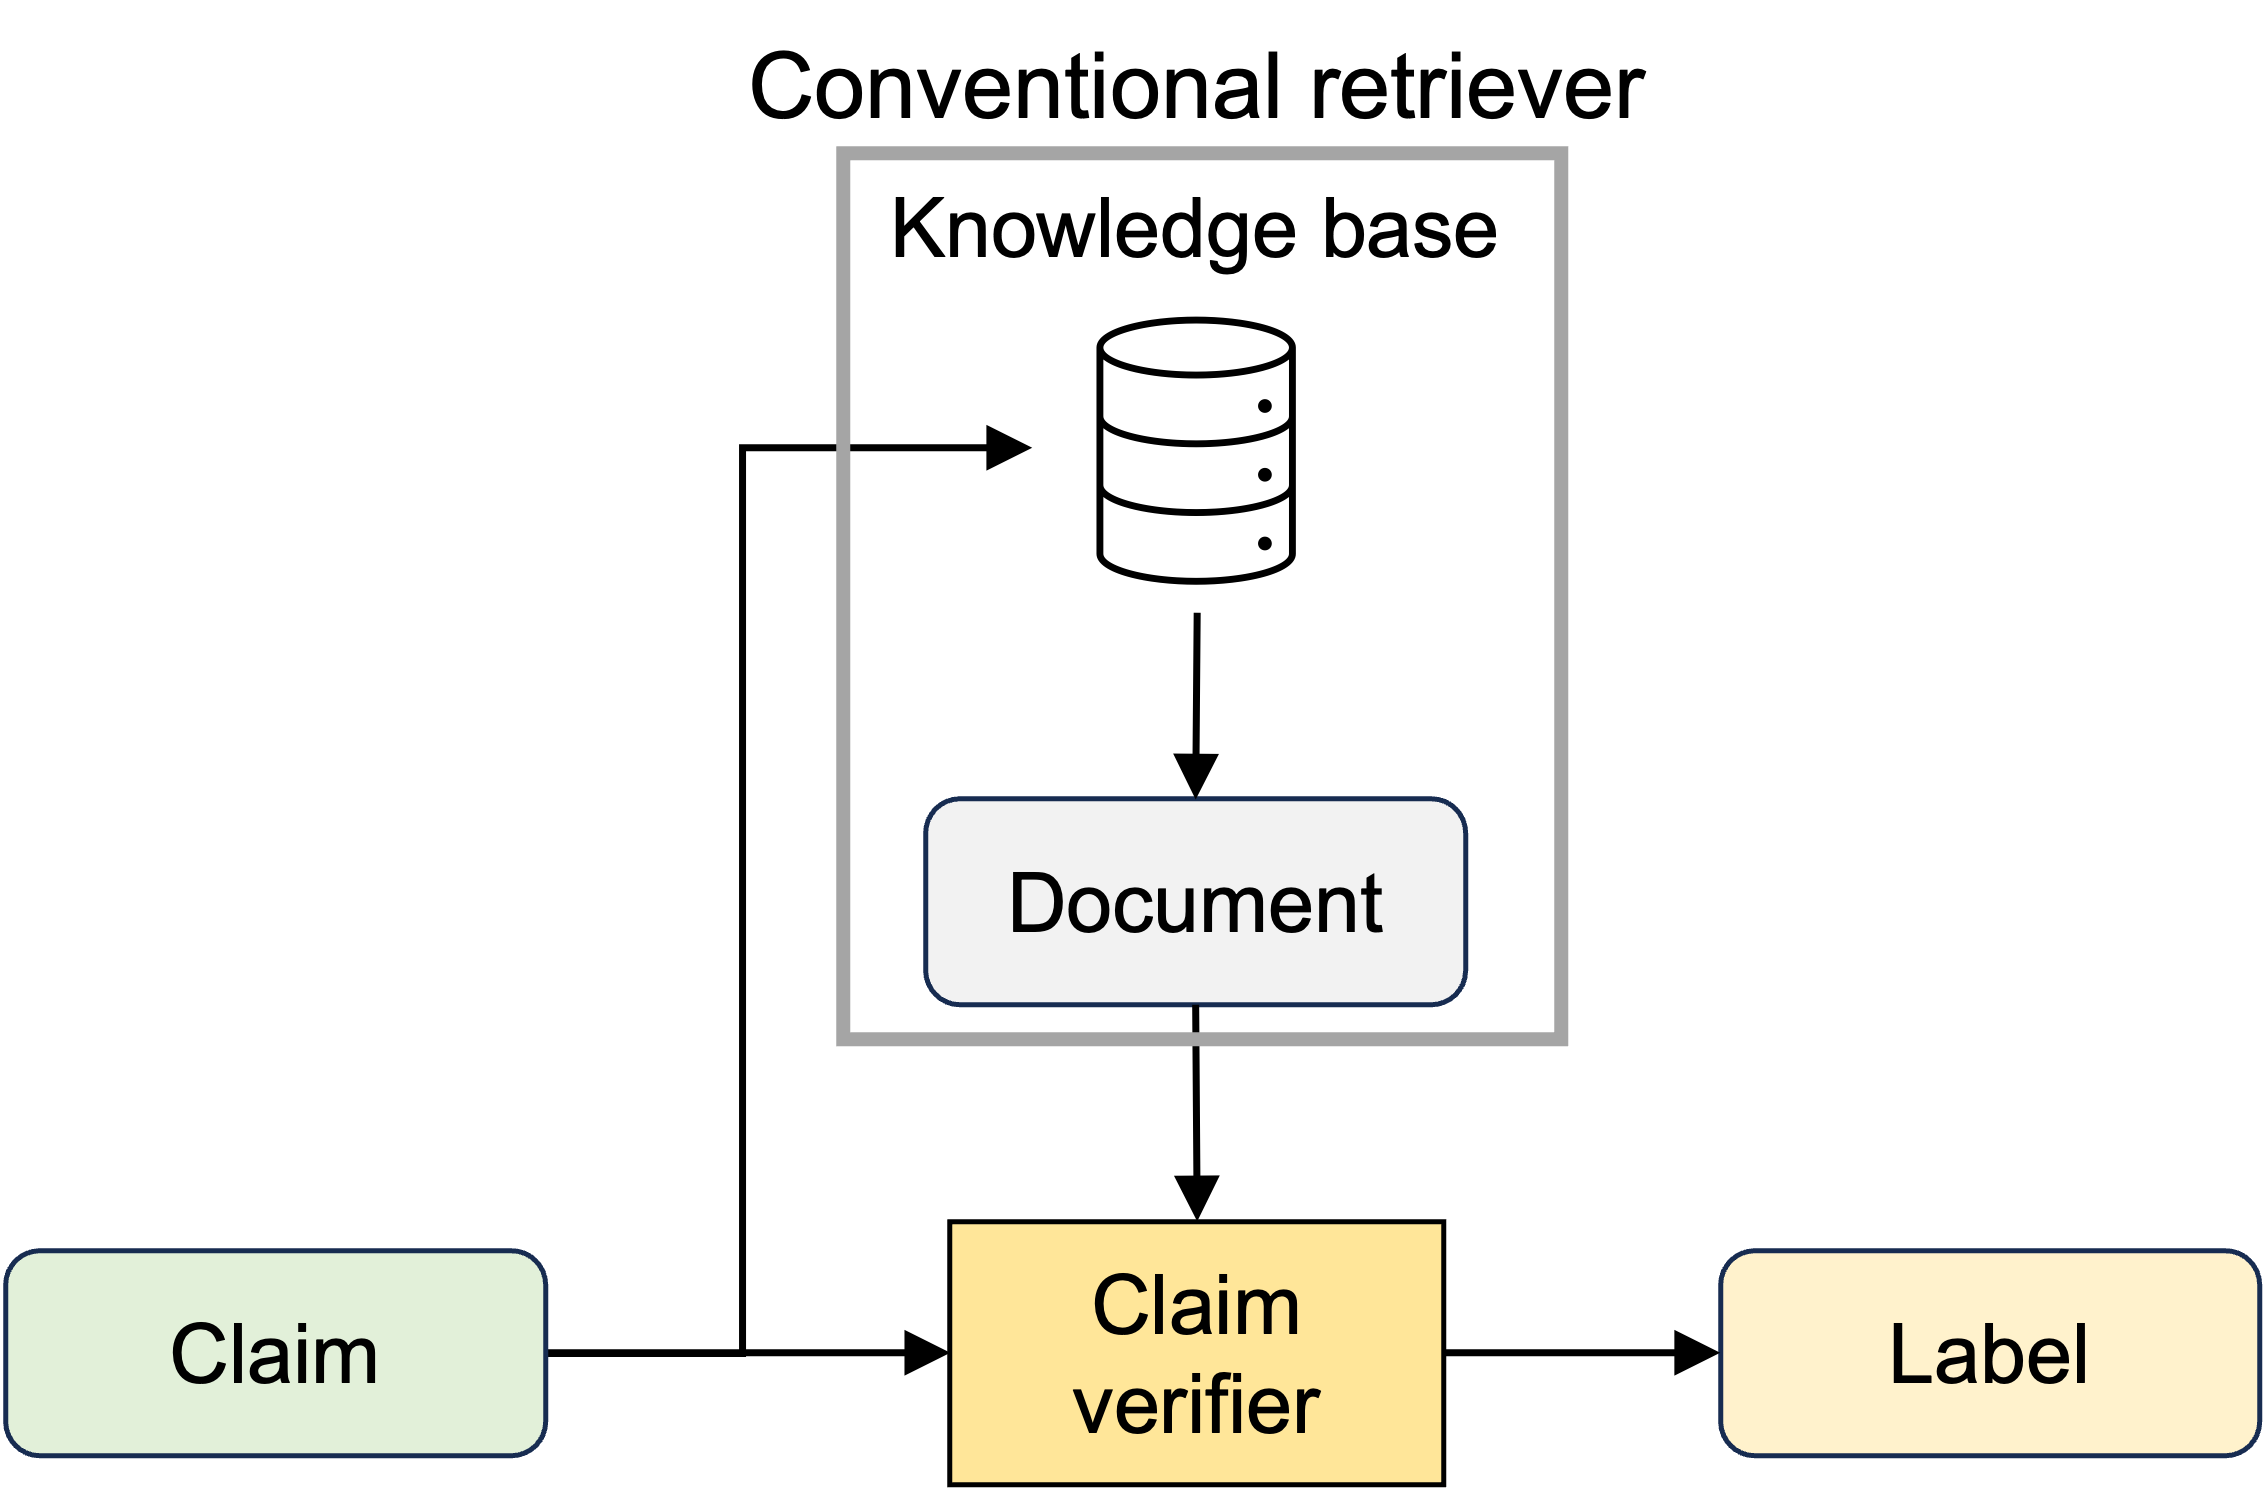
\includegraphics[width=0.45\linewidth]{Figure/Fig1.png}
  \caption{\label{bl}Baseline Model Architecture}
\end{figure}\begin{figure}[h]
  \centering
  \includegraphics[width=0.8\linewidth]{Figure/Fig2.png}
  \caption{\label{pp}Proposed Model Architecture}
\end{figure}

\subsection{Baseline model}
Baseline model consists of retriever and claim verifier. The retriever first retrieves the documents that are similar to given claim, by querying to the knowledge base. Claim and retrieved documents are put into the claim verifier, which then returns the factuality label (True, False, or Not Verifiable).
\subsubsection*{Experiment with baseline model}
Our baseline model is constructed based on LlamaIndex \cite{LlamaIndex}, a framework for LLM-based application. Wikipedia documents from FEVER dataset (5,416,537 documents) are stored in vector database (pgvector on PostgresSQL), after transformed to embedding vectors. BAAI’s embedding model \cite{bge_embedding} is used as sentence transformer. When a claim is given, it is transformed to a query embedding. Then, the documents are retrieved from the knowledge base based on the similarity with the query embedding. Claim and contexts (retrieved documents) are fed to Llama 2 \cite{touvron2023llama} model with fact-checking prompt. The baseline model is tested on claim samples from FEVER and HOVER datasets. It should be noted that HOVER dataset has only two labels (Supported and Not supported) because of ambiguity between False and Not Verifiable in multi-hop claims. It is clearly shown that the conventional retrieval model fails to correctly verify the claims with multi-hop.

\begin{table}[h]
  \centering
  \begin{tabular}{c|c|ccc}
  \toprule
           & FEVER & \multicolumn{3}{c}{HOVER} \\ \midrule
           & 1-hop & 2-hop   & 3-hop  & 4-hop  \\ \midrule
  EM       & 0.49  & 0.44    & 0.44   & 0.41   \\
  F1 score & 0.47  & 0.55    & 0.43   & 0.39   \\ \bottomrule
  \end{tabular}\\[5pt]
  \caption{Baseline model performance on FEVER and HOVER datasets}
\end{table}

\subsection{Subclaim generator}
The subclaim generator in QACHECK plays a crucial role in breaking down complex claims into contextually relevant subclaims, using InstructGPT. This process generates essential initial and subsequent follow-up questions, which are integral to the system's multi-hop reasoning approach. This method ensures a comprehensive and thorough fact-checking process.

\subsection{Generative retriever}
The generative retriever consists of 3 independent components, including claim encoder, title decoder and evidence decoder. It first encodes the claim into a compact vector to capture its essential topics. Then the title decoder predicts a sequence of document titles based on both the claim and previous generated titles. Generated titles are used to retrieve relevant documents which contributes candidate sentence set. The sentence set are used to predict sentence identifier, which generates a dynamic set of evidence.

\subsection{Evaluation}
To evaluate the fact verification performance of the proposed model, we will use the fact verification datasets: FEVER, HOVER \cite{jiang2020hover}, and FEVEROUS \cite{aly2021feverous}. They are open-domain fact verification dataset based on Wikipedia articles. While FEVER mostly has single-hop claims (related to a single document), HOVER and FEVEROUS have multi-hop claims (related to multiple documents). F1 score will be used as evaluation metric.
Other sub-tasks and evaluation metrics will be proposed in further study: e.g., performance of subclaim generation, performance of generative retrieval, memory efficiency in knowledge base storage, and time-efficiency in inference.


\section{Future Work and Improvement}

\subsection{Integrating Subclaim Generation from QACHECK into baseline model}
Our primary objective is to enhance the capability of our existing NLP system especially in the claims generators parts, through the integration of QACHECK. This integration aims to leverage the sophisticated, question-guided multi-hop reasoning mechanism of QACHECK for more effective and interpretable fact-checking processes within our NLP tasks.\par
We will align current retrieval component with QACHECK’s subclaim generation module. This will involve modifying the retrieval process to utilize the output of the subclaim generator to get more effective information retrieval. The integration will require modifying the data flow process so that the input to the subclaim generator comes directly from the LlamaIndex’s output. Then, subclaims generated by QACHECK will be fed back into LlamaIndex’s retrieval and embedding modules. This can create a recursive retrieval process, enhancing the overall relevance and accuracy of the information gathered. \par
While Instruct GPT is effective in generating contextually relevant questions,  but integrating transformer models like BERT or GPT-3 could provide additional improvements. These have advanced capabilities in understanding nuances and complex language structures, which can lead more precise and varied subquestions.

\subsection{Integrating GERE as a retriever module to our baseline model}
In our pursuit of generating evidence that is not only more flexible and aligned with factual accuracy but also ensuring improved time-efficiency and memory-efficiency, we are strategically incorporating the GERE into our processing system as a dedicated retriever module.While GERE can be easily adapted to our claim verification model, there also remain some space for future improvement. By incorporating additional contextual information during the sentence prediction step, GERE could capture a more comprehensive set of relevant evidence. By seamlessly integrating GERE, we aim to enhance the speed, and resource utilization of our fact-validation system, thereby advancing its effectiveness in delivering precise and reliable results in a timely and resource-conscious manner.

\bibliographystyle{unsrt}
\bibliography{References}

\end{document}